% Document meta
\documentclass[12pt]{article}
\usepackage[a4paper, includeheadfoot, margin = 1.5cm]{geometry}
\usepackage[unicode=true, colorlinks=true, linkcolor=black, urlcolor=black]{hyperref}

% Bulgarian
\usepackage[T1, T2A]{fontenc}
\usepackage[utf8]{inputenc}
\usepackage[bulgarian]{babel}

\usepackage{csquotes}

% Better tables
\usepackage{array}
\usepackage{multirow}
\usepackage{tabularx}
\usepackage{tablefootnote}
 
% Ensure images stay in their section
\usepackage{placeins}

% Easier text formatting
\usepackage{indentfirst}
\usepackage{ulem}
\usepackage{xcolor}

\usepackage{comment}
\usepackage{enumitem}

% Math
\usepackage{amsmath,amssymb}
\usepackage{mathtools}
\usepackage{mathptmx}
\usepackage{tikz}
\usepackage{bm}

% Code
\usepackage{minted} % REQUIRES PYGMENTS: pip install Pygments
\usepackage{listings}

\lstset{frameround=fttt,language=R,numbers=left,breaklines=true}

\selectlanguage{bulgarian}

%\fontsize{16pt}{20pt}\selectfont
\renewcommand{\sfdefault}{cmss}
\renewcommand{\rmdefault}{cmr}
\renewcommand{\ttdefault}{cmt}

\renewcommand{\thesection}{\Roman{section}} 
%\renewcommand{\thesubsection}{\thesection.\Roman{subsection}}

% Mono font for function names
\newcommand{\code}{\texttt}

\newcommand\numberthis{\addtocounter{equation}{1}\tag{\theequation}}

\newcolumntype{L}[1]{>{\raggedright\let\newline\\\arraybackslash\hspace{0pt}}m{#1}}

\renewcommand{\footnoterule}{% Kerns avoid vertical space
  \kern -3pt                         % This -3 is negative
  \hrule width \textwidth height 1pt % of the sum of this 1
  \kern 2pt}                         % and this 2
  
\title{Статистически анализ на данни от кръвта на атлети}
\author{Калоян Стоилов}

\begin{document}

\begin{titlepage}

\begin{center}
	\begin{Huge}
       \textbf{Статистически анализ на данни от кръвта на атлети}
       \\
	\end{Huge}
	\vspace{0.5cm}
	\begin{Large}
	проект по \\ Вероятности и статистика
	\end{Large}
      \end{center}      
       \vspace{5cm}

		\begin{flushleft}
		\begin{Huge}
		\textbf{Изготвил: Калоян Стоилов, ф.н. 81609, спец. КН, курс 3, група 5}
		\end{Huge}
		\end{flushleft}
		\begin{Large}
	\begin{center}
	\vfill
   \textbf{\textit{СОФИЙСКИ УНИВЕРСИТЕТ \\ "СВ. КЛИМЕНТ ОХРИДСКИ"}}
   

   	       
   	
\includegraphics[width=3.5cm,height=4.5cm]{logo_su_s_nadpis_imagelarge}
   	\\
   	{\Large \textbf{ФАКУЛТЕТ ПО МАТЕМАТИКА И ИНФОРМАТИКА}}
   	\\
       
	\end{center}  
	   \end{Large}

\end{titlepage}

\begin{large}
\tableofcontents{}


\section{Информация за данните}
Данните са взети от Rdatasets, Package DAAG, Item ais \footnote{Може да ги свалите от този URL: \url{https://vincentarelbundock.github.io/Rdatasets/csv/DAAG/ais.csv}}. Данните са относно австралийски атлети от различни дисциплини и са направени измервания на различни характеристики(концентрация червени/бели кръвни телца, маса, пол, спорт и т.н.). За целите на поставената задача се ограничаваме до изследване на номиналната категорийната променлива пол(\textit{sex}) с възможни стойности \textbf{мъж}(m) и \textbf{жена}(f), както и на двете непрекъснати числови променливи: маса без масата на мастната тъкан(още известна като LBM) в \textbf{кг}(\textit{lbm}); концентрация на бели кръвни телца в \textbf{$10^9$ за литър}(\textit{wcc}). \par
Ще отбележим, че \uline{няма повторни измервания}, тъй като при тях има ограничения на множеството използваеми статистически тестове.

\section{Цели на проекта}

В проекта ще направим таблично и/или графично представяне на основните статистики и данните. Опитваме да отговорим на следните въпроси:

\begin{itemize}
\item Нормално разпределени ли са LBM и концентрацията на бели кръвни телца при атлетите (въобще, при мъжете и при жените)?
\item Има ли статистически значима разлика между концентрацията на бели кръвни телца при мъжете и жените атлети?
\item Има ли статистически значима разлика между LBM при мъжете и жените атлети?
\item Има ли корелация между концентрацията на бели кръвни телца и LBM при атлетите (въобще, при мъжете и при жените)?
\item Има ли регресионна права за предвиждане на концентрацията на белите кръвни телца чрез LBM?
\end{itemize}

\section{Статистики}
За получаванете им са използвани вградените в R функции \code{mean}, \code{median}, \code{sd} и \code{var}. Тъй като в R не е вградена функция за мода на извадка, е използвана предоставената във упражнение функция modeFunction с малка промяна, за да връща реално число.

\begin{minted}[mathescape,
               linenos,
               numbersep=5pt,
               frame=none,
               framesep=2mm]{R}
	modeFunction <- function(x) {
		tt <- table(x)
		return(as.double(names(tt)[tt==max(tt)]))
	}
\end{minted}

За бройките съответно на всички атлети и отделните полове използваме вградените фунции length и table. Атлетите са \textcolor{green}{$202$}, като \textcolor{pink}{$100$} от тях са жени, а \textcolor{blue}{$102$} - мъже.

За взимане само на записите за отделен пол използваме:
\begin{minted}[mathescape,
               linenos,
               numbersep=5pt,
               frame=none,
               framesep=2mm]{R}
	aisf=ais[ais$sex == 'f',]
	aism=ais[ais$sex == 'm',]
\end{minted}
Така достигнахме до следната таблица с дескриптивни статистики:
\clearpage

\begin{table}
\centering
\begin{tabular}{ |L{3cm}|L{2.4cm}|L{2.4cm}|L{2.4cm}|L{2.4cm}|L{2.4cm}|  }
 \hline 
 Извадка & Средна & Медиана & Мода \tablefootnote{Зачитаме, че при повече от една най-често срещана стойност, и тя е мода.} & Дисперсия & Стандартно отклонение\\
 \hline \hline
 LBM-всички & 64.87371 & 63.035 & 78 & 170.8301 & 13.0702 \\
 \hline
 Конц. бели кръвни телца-всички & 7.108911 & 6.85 & 6.4 & 3.241214 & 1.800337 \\
 \hline
 LBM-мъже & 74.656863 & 74.5 & 78 & 97.752378 & 9.886980 \\
 \hline
 Конц. бели кръвни телца-мъже & 7.221569 & 7.1 & 7.5 и 8.9 & 3.606857 & 1.899173 \\
 \hline
 LBM-жени & 54.8949 & 54.92 & 53.11, 53.2 и 56.05 & 47.916748 & 6.922192 \\
 \hline
 Конц. бели кръвни телца-жени & 6.994000 & 6.7 & 6.4 & 2.874509 & 1.695438 \\
 \hline
\end{tabular}
\caption{Таблица с дескриптивни статистики}
\end{table}

\section{Хистограми}
Хистограмите са изпечатани с написана функция hister(картината долу), използваща вградените \texttt{hist} и axis. Причината е, че базово интервалите на x координатата зависят от предоставената информация. Така е и с краищата ѝ. Това обаче може да даде грешна представа за разположението на подмножествата от данните за двата пола(едно спрямо друго, както и спрямо данните от всички атлети). Поради желанието за еднакви краища и интервали навсякъде, за всяка от числовите променливи се решава какви да са те, в зависимост от минималните и максималните стойности при всички. 

\begin{minted}[mathescape,
               linenos,
               numbersep=5pt,
               frame=none,
               framesep=2mm]{R}
hister<-function(info, mname, xname, yname, hcol, xl, yl, xm, ym, xint, yint, brnum){
  hist(info, main=mname, xlab=xname, ylab=yname, col=hcol,
   	breaks = brnum, xlim=c(xl,xm), ylim=c(yl,ym))
  axis(side=1,at=seq(xl,xm,xint))
  axis(side=2,at=seq(yl,ym,yint))
}
\end{minted}

\clearpage

\subsection{Хистограми на LBM}

\begin{figure}[h!]
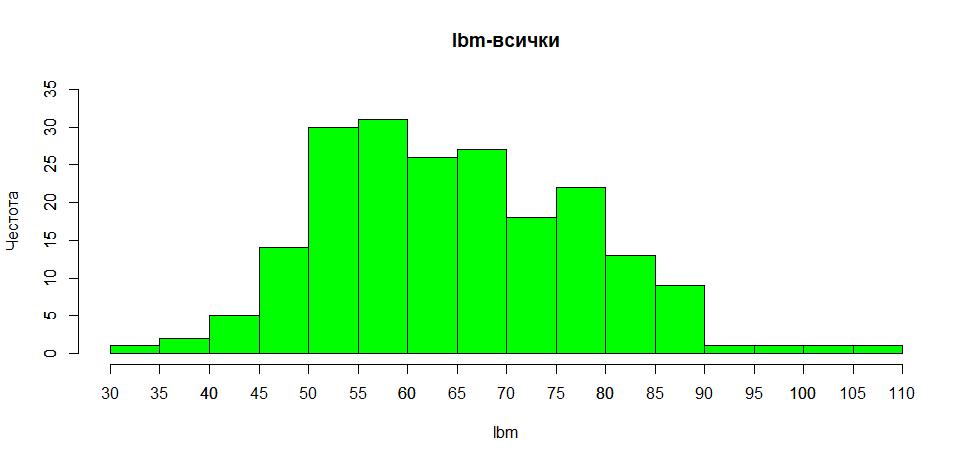
\includegraphics[width=\textwidth,height=\textheight,keepaspectratio]{pics/lbmall}
\caption{Хистограма на маса без масната тъкан за всички атлети}
\end{figure}

\begin{figure}[h!]
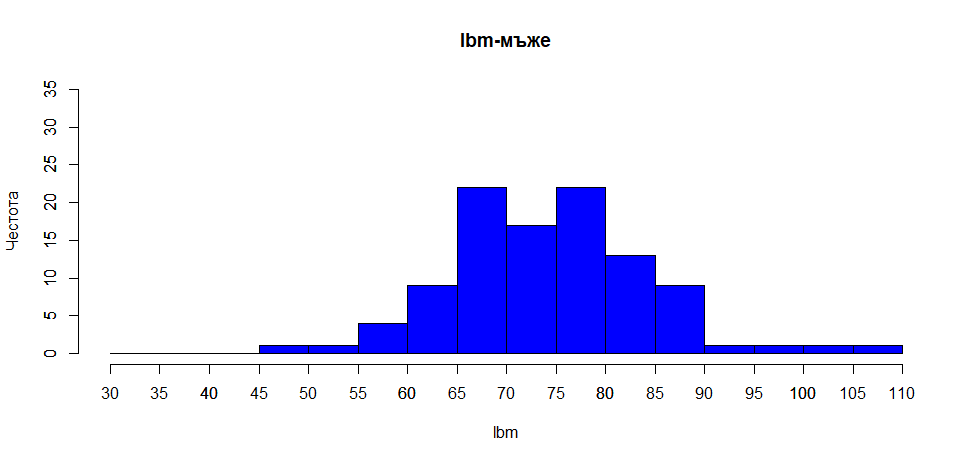
\includegraphics[width=\textwidth,height=\textheight,keepaspectratio]{pics/lbmmen}
\caption{Хистограма на маса без масната тъкан за мъжете атлети}
\end{figure}

\begin{figure}[h!]
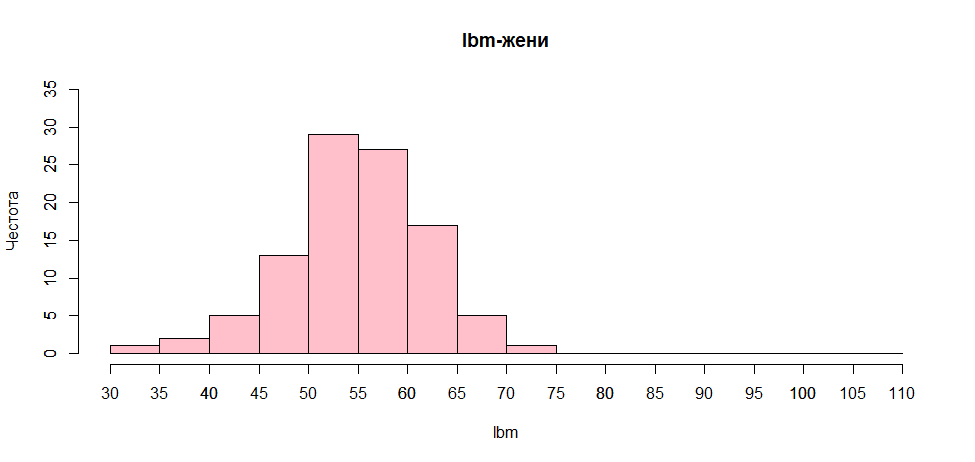
\includegraphics[width=\textwidth,height=\textheight,keepaspectratio]{pics/lbmwomen}
\caption{Хистограма на маса без масната тъкан за жените атлети}
\end{figure}

\FloatBarrier
\subsection[Хистограми на концентрации на бели кръвни телца]{Хистограми на концентрации на бели кръвни телца\footnote{Поради възникнали проблеми с визуализацията на хоризонталната ос при разделители реални числа, тя е разграфирана през 1, а интервалите за хистограмата са с дължина 0.5.}}
\FloatBarrier

\begin{figure}[h!]
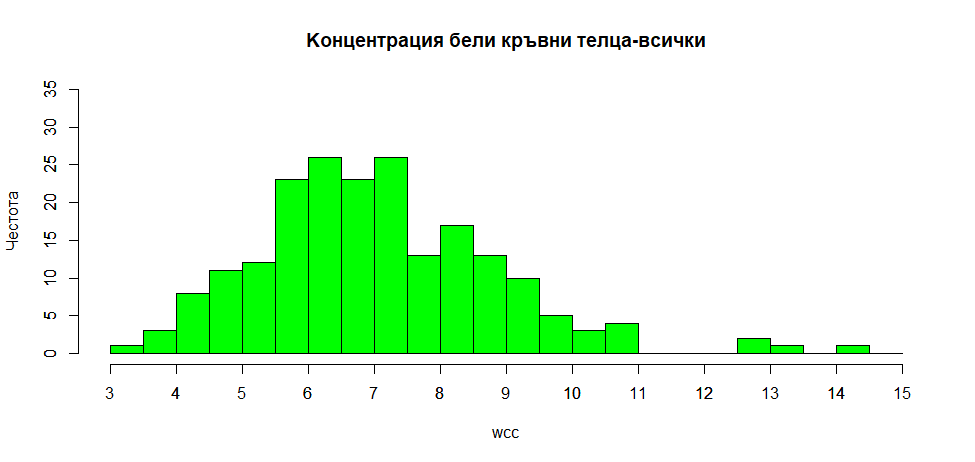
\includegraphics[width=\textwidth,height=\textheight,keepaspectratio]{pics/wccall}
\caption{Хистограма на концентрацията на бели кръвни телца за всички атлети}
\end{figure}

\begin{figure}[h!]
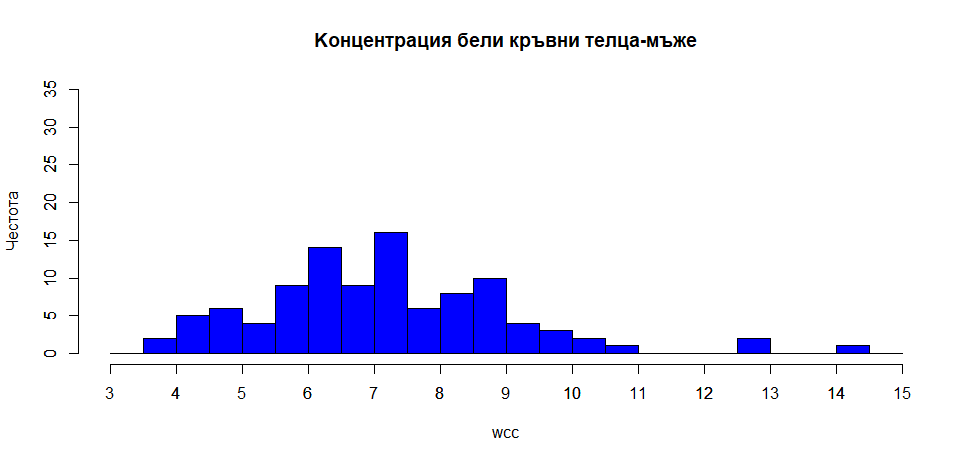
\includegraphics[width=\textwidth,height=\textheight,keepaspectratio]{pics/wccmen}
\caption{Хистограма на концентрацията на бели кръвни телца за мъжете атлети}
\end{figure}

\begin{figure}[h!]
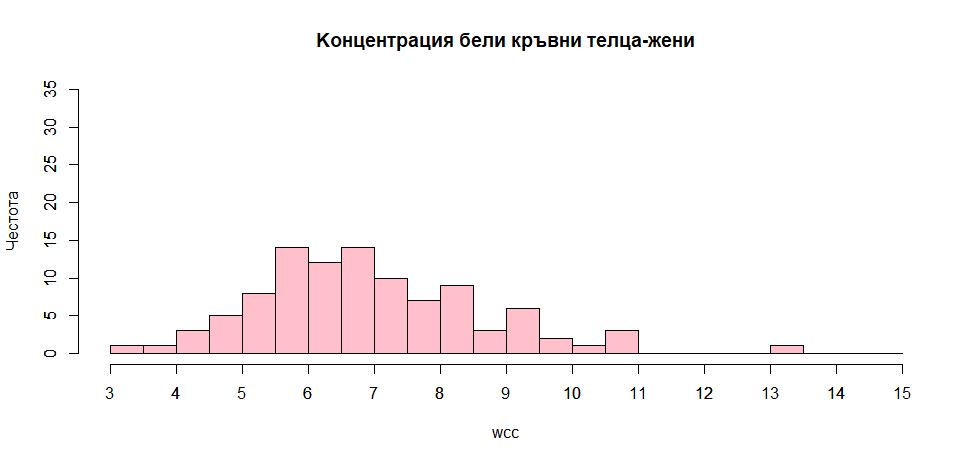
\includegraphics[width=\textwidth,height=\textheight,keepaspectratio]{pics/wccwomen}
\caption{Хистограма на концентрацията на бели кръвни телца за жените атлети}
\end{figure}

\section{Изследване на разпределенията}

\subsection{Нормална разпределеност}
Тук изследваме дали извадките са нормално разпределени, чрез тестът на Shapiro-Wilcoxon(с $\alpha=0.05$). Използвана е вградената функция shapiro.test. Резултатите са представени в следната таблица:

\begin{table}[h!]
\centering
\begin{tabular}{|l|l|l|}
 \hline 
 Извадка & p & Нормално разпределена\\
 \hline \hline
 LBM-всички & 0.1286 & Не \\
 \hline
 Конц. бели кръвни телца-всички & 0.00002591 & Не \\
 \hline
 LBM-мъже & 0.2175 & Да \\
 \hline
 Конц. бели кръвни телца-мъже & 0.01237 & Не \\
 \hline
 LBM-жени & 0.468 & Да \\
 \hline
 Конц. бели кръвни телца-жени & 0.001129 & Не \\
 \hline
\end{tabular}
\caption{Таблица с резултати от теста за нормална разпределеност}
\end{table}

\subsection{Сравнение на LBM при двата пола атлети}

Тъй като LBM при мъжете и жените са нормално разпределени, може да приложим t-тест на Welch за тяхно сравнение. От хистограмата изглежда, че може би LBM при мъжете е с по-голяма средна. За това решаваме тестът да е с:
\begin{description}
\item[$H_0$] Мъжете и жените атлети имат еднакви средни стойности LBM. 
\item[$H_1$] Средната стойност на LBM при мъжете атлети е по-голяма от тази на жените атлети.
\end{description}
Тоест правим едностранен t-тест, като нека $\alpha=0.05$. Използвайки вградената в R функция t.test, достигаме до резултат $\mathbf{p<2.2 \times 10^{-16}}$. Нулевата хипотеза се отхвърля. Достигаме до заключението, че \uline{има статистически значима разлика между LBM при мъжете и жените атлети, като средностатистически мъжете атлети имат по-голям LBM}.

\subsection{Сравнение на концентрацията на бели кръвни телца при двата пола атлети}
Видяхме, че концентрациита на бели кръвни телца при двата пола не 
са разпределени нормално. Поради това не може да използваме t-тест за 
тяхното сравнение. Ще се наложи да използваме някой непараметричен 
тест. Тъй като броят на тествани мъже е различен от този на жените, ще 
приложим тестът Mann-Whitney U/Wilcoxon rank sum:
\begin{description}
\item[$H_0$] Няма разлика между концентрациите на бели кръвни телца при мъжете и жените атлети. 
\item[$H_1$] Налице е разлика между концентрациите на бели кръвни телца при мъжете и жените атлети.
\end{description}
Тоест правим двустранен U тест, като нека $\alpha=0.05$. Използвайки 
вградената в R функция wilcox.test, достигаме до резултат $\mathbf{p=0.3853}$. 
Нулевата хипотеза не се отхвърля. Достигаме до заключението, че \uline{няма статистичеси значима разлика между концентрациите на бели кръвни телца при мъжете и жените атлети}.


\section{Зависимости между LBM и концентрацията на бели кръвни телца при атлетите}

\subsection{Корелационни коефициенти}
Използваме вградената функция cor, за да получим корелацията 
между LBM и концентрацията на белите кръвни телца при всички атлекти, както и само при мъжете и само при жените. Резултатите са представени в следната таблица:

\begin{table}[h!]
\centering
\begin{tabular}{|l|l|l|}
 \hline 
 Извадка & Корелационен коефициент & Интерпретация\\
 \hline \hline
 Всички & 0.1026625 & Много слаба положителна корелация \\
 \hline
 Мъже & 0.1067 & Много слаба положителна корелация \\
 \hline
 Жени & 0.04830104 & Няма корелация \\
 \hline
\end{tabular}
\caption{Таблица с корелационни коефициенти}
\end{table}

\subsection{Диаграми на разсейване и регресия}
За да представим зависимостта, ще използваме написана от нас функция scatterer, показана по-долу, като функциите, използвани в дефиницията ѝ са само вградени. Тя рисува диаграма на разсейването с plot. След това намира линейна регресия чрез lm. Ако регресията е статистически значима, чертае графиката ѝ, а иначе изпечатва противното в конзолата.

\begin{minted}[mathescape,
               linenos,
               numbersep=5pt,
               frame=none,
               framesep=2mm]{R}
scatterer<-function(info1, info2, mname, xname, yname, scol,
                    	xl, yl, xm, ym, xint, yint, alpha){
  plot(info1, info2, main=mname, xlab=xname, ylab=yname, col=scol,
       xlim=c(xl, xm),ylim=c(yl, ym))
  axis(side=1, at=seq(xl, xm, 2*xint))
  axis(side=2, at=seq(yl, ym, 2*yint))
  
  regression=lm(info2~info1)
  regsum=summary.lm(regression)
  pvalue=regsum$coefficients[2, 4]
  
  if(pvalue<=alpha) abline(regression,col=scol)
  else print("Linear regression is not significant")
}
\end{minted}

\begin{figure}[!h!]
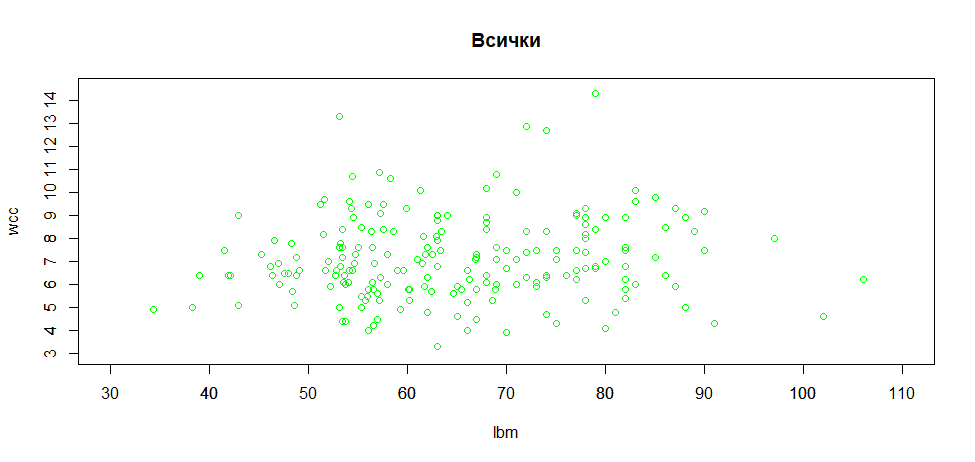
\includegraphics[width=\textwidth,height=\textheight,keepaspectratio]{pics/scatterall}
\caption{Диаграма на разсейването за всички атлети}
\end{figure}

\begin{figure}[!h!]
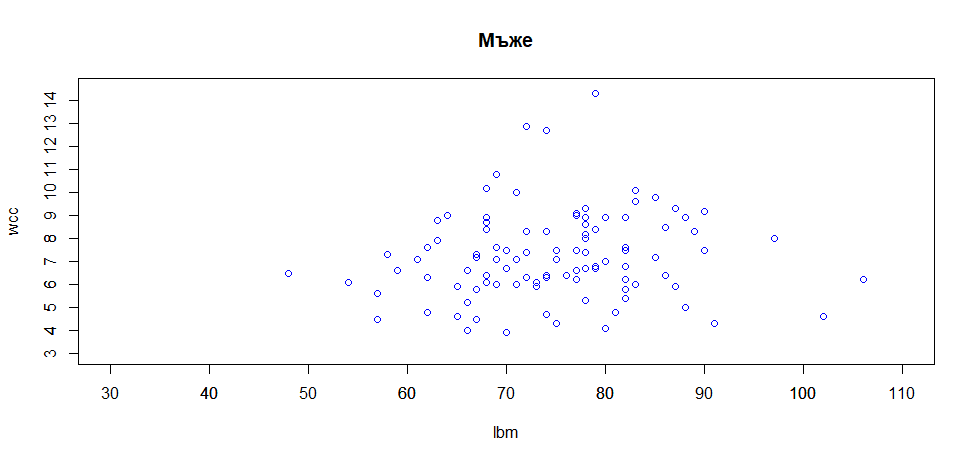
\includegraphics[width=\textwidth,height=\textheight,keepaspectratio]{pics/scattermen}
\caption{Диаграма на разсейването за мъжете атлети}
\end{figure}

\clearpage
\begin{figure}[!h!]
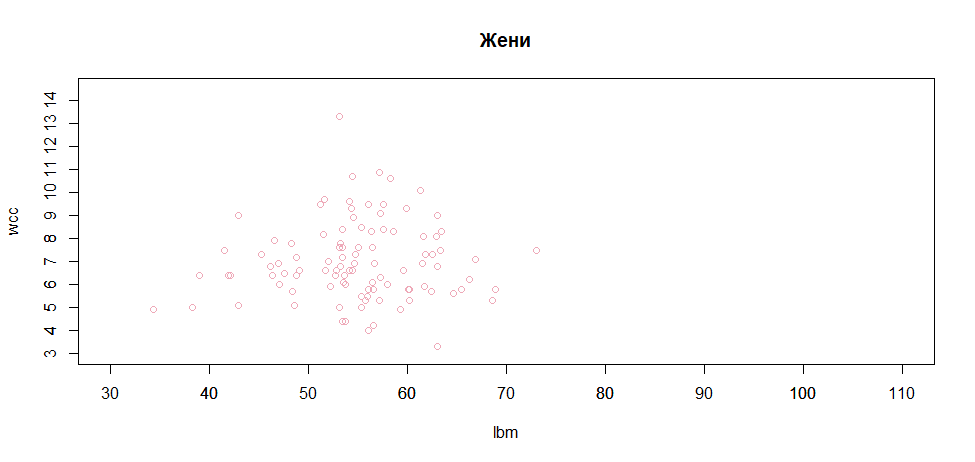
\includegraphics[width=\textwidth,height=\textheight,keepaspectratio]{pics/scatterwomen2}
\caption{Диаграма на разсейването за жените атлети}
\end{figure}

Диаграмите показват, че \uline{между LBM и концентрацията на бели кръвни телца няма статистически значима линейна зависимост} (при ниво на значимост $\alpha=0.05$). \par
Съдейки по формата на диаграмите на разсейване, по-скоро няма функционална зависимост от какъвто и да било тип.

\section{Заключение}
Следните заключения правим при  разумното предположение, че няма някаква голяма разлика във физическото устройство между австралийските атлети и атлетите от другите страни. \par
На база на представените данни може да твърдим \footnote{Хистограми на концентрации на бели кръвни телца}, че:
\begin{enumerate}
\item LBM при мъжете и жените атлети отделно е норманло разпределен, но не е, ако ги разглеждаме заедно, като средностатистически атлет от мъжки пол има по-голям LBM.
\item Концентрацията на белите кръвни телца не е нормално разпределена при атлетите, дори и разглеждайки половете поотделно. Няма разлика в концентрацията на белите кръвни телца между двата пола.
\item Между LBM и концентрацията на белите кръвни телца при атлетите няма забележима корелация. Регресионна права за изразяване на концентрацията на белите кръвни телца чрез LBM няма.
\end{enumerate}

\addcontentsline{toc}{section}{\listfigurename}
\listoffigures

\addcontentsline{toc}{section}{\listtablename}
\listoftables

\end{large}
\end{document}
